\section{Methodology}

\begin{figure*}[t!]
  \centering
   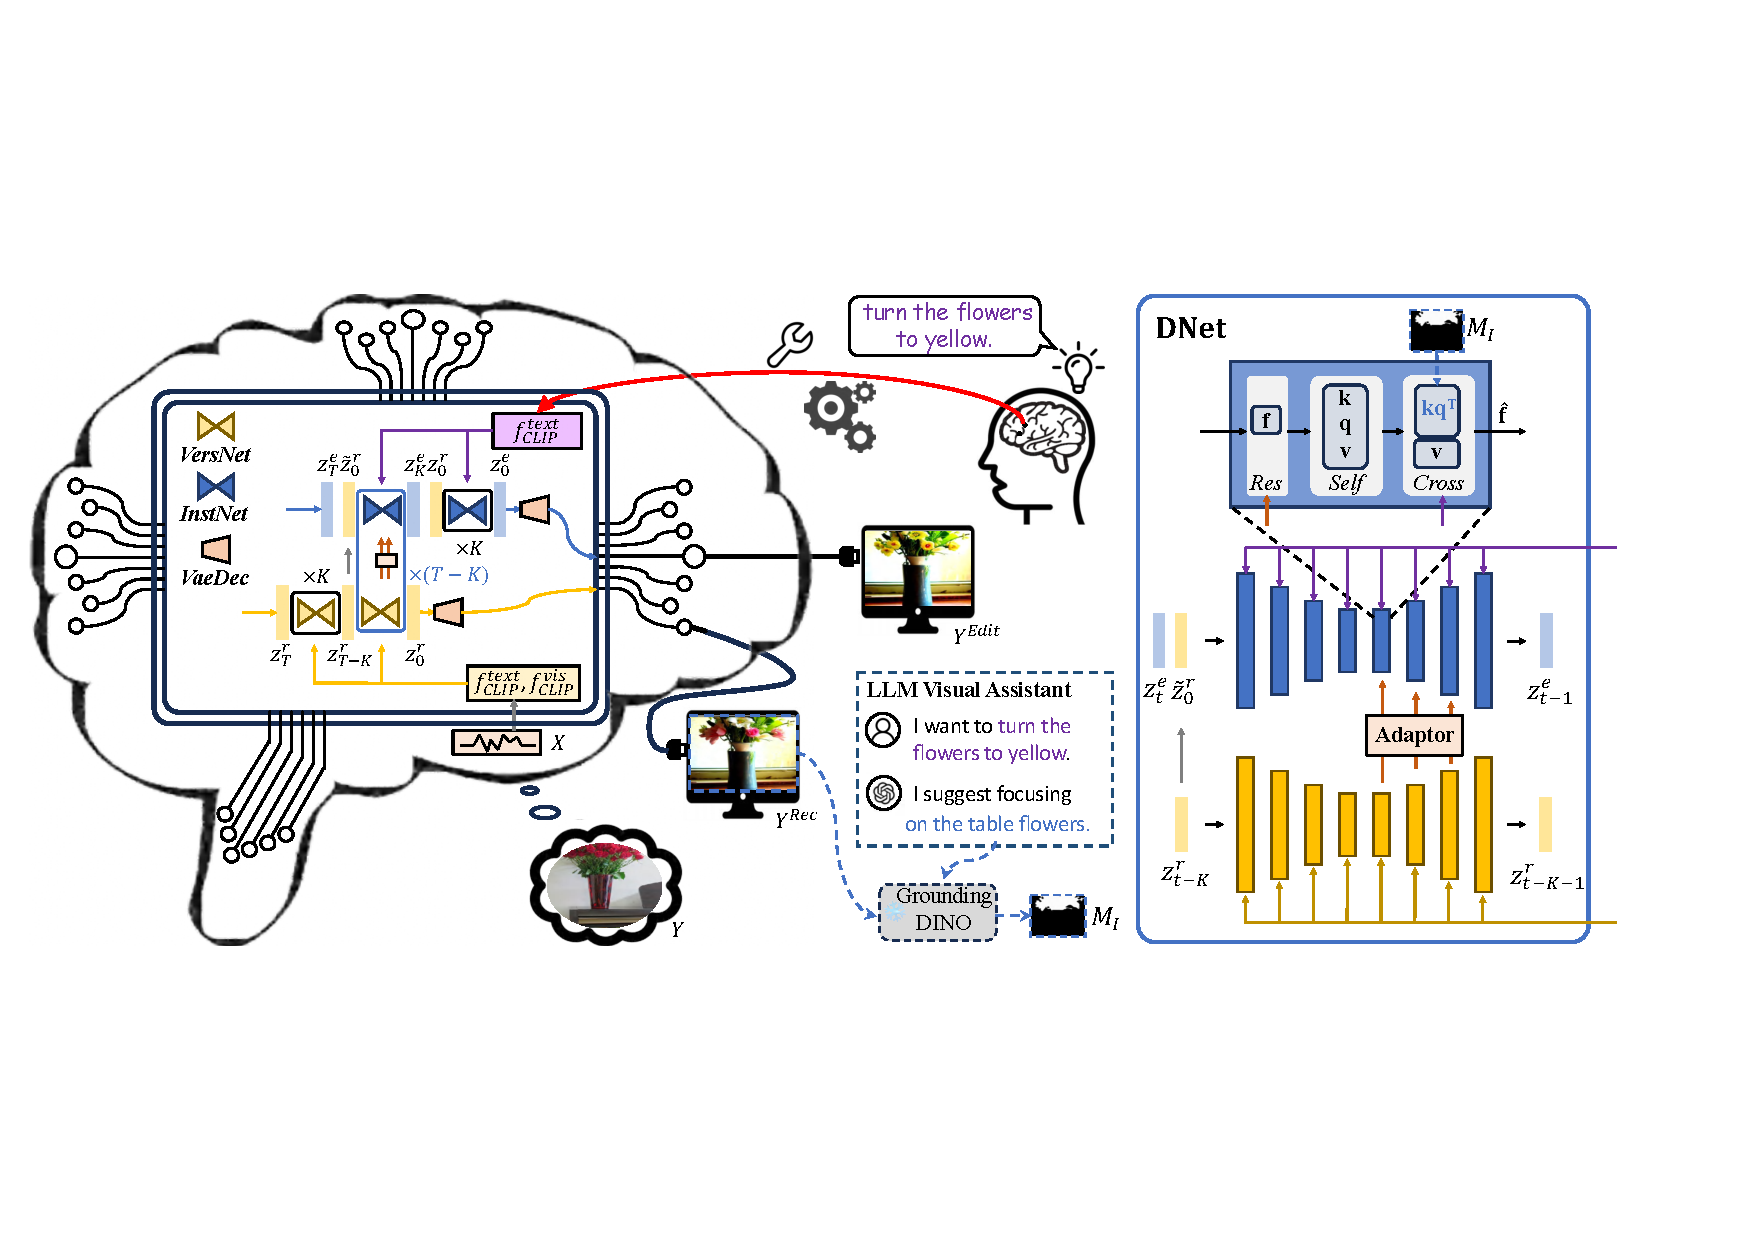
\includegraphics[width=\linewidth]{figs/arch5.pdf}
  \caption{\textbf{Illustration of the proposed \textbf{\model{}} framework.}
    A person's biological signal indicated by fMRI sequences $X$, will be activated within his brain according to his ``dreams'' represented by the visual stimuli $Y$.
    Our system targets to interface with $X$ via a natural language instruction $I$.
    Specifically, the fMRI signal is regressed to CLIP text and visual embedding, $f_{\text{CLIP}}^{text}$ and $f_{\text{CLIP}}^{vis}$, which are leveraged to aligned with visual content $z^r_t$ in \emph{\textbf{VersNet}}~\cite{xu2023versatile}. After modulated by an adaptor, its intermediate spatial features are fed to \emph{\textbf{InstNet}}~\cite{geng2023instructdiffusion}. Encoded by CLIP text encoder, the human instruction $I$ is injected to \emph{\textbf{InstNet}} to modulate these features toward intended direction.
  }
  \label{fig:arch}
\end{figure*}



In this section, we discuss the details of the proposed \emph{Visual Brainstorming Instruction System}, termed \textbf{\model{}}. The primary objective of this framework is to develop a model capable of providing instruction in brain activity. To achieve this, the model must possess the ability to associate human instructions with fMRI signal and modify its embedded pertinent visual information. The overall pipeline is depicted in Fig.~\ref{fig:arch} where we devise an asynchronous dual-stream diffusion architecture coupled with an adaptor to promote \emph{progressive interpretation and instruction}. To facilitate faithful instruction within pertinent regions from both temporal and spatial perspectives, we introduce an asynchronous diffusion strategy and an LLM-guided region-aware manipulation operation.

\subsection{Dual Stream Diffusion Instruction}
\textbf{Problem Formulation.} Given a visual stimuli $Y \in \mathcal{R}^{3 \times H \times W}$, a person's biological signal revealed by fMRI, $X \in \mathcal{R}^{N_f}$, will be activated, where ${N_f}$ represents the number of relevant voxels. The traditional image reconstruction task targets to recover its indicted visual content $Y^{Rec}$ from $X$. In contrast, we study directly manipulating the entailed information to $Y^{Edit}$ following a piece of natural language instruction $I$.
Accomplishing this objective requires a comprehensive cross-modal association between the fMRI signal and the specified instruction. To resolve this issue, we leverage the rich contextual prior within StableDiffusion (SD) to bridge the modality gap due to its effective exploitation in numerous visual tasks. The key is to derive a unified diffusion framework to tackle feature alignment and interaction among distinct modalities progressively.

\paragraph{Preliminary on Diffusion Models.}
Diffusion models~\cite{ho2020denoising} stand out due to its stable training objective and exceptional ability to generate high-quality images. It operates by iteratively denoising Gaussian noise to produce the image $\bm{x}_0$.
Typically, the diffusion model assumes a Markov process~\cite{rabiner1989tutorial} wherein Gaussian noises are gradually added to a clean image $\bm{x}_0$ based on the following equation:
\begin{equation}
    \bm{x}_t = \sqrt{\alpha_t} {\bm{x}}_{0} + \sqrt{1-\alpha_t} \bm{\epsilon} ,
\label{eq:forward}
\end{equation}
where $\bm{\epsilon}\!\sim\!\mathcal{N}(0, \mathbf{I})$ represents the additive Gaussian noise, $t$ denotes the time step and $\alpha_t$ is scalar functions of $t$.
Our objective is to devise
a neural network $\bm{\epsilon}_\theta(\bm{x}_t, t, c)$ to predict the added noise $\bm{\epsilon}$.
Empirically, a simple mean-squared error is leveraged as the loss function:
\begin{equation}
    L_{simple} := \mathbb{E}_{\bm{\epsilon} \sim \mathcal{N}(0, \mathbf{I}), \bm{x}_0, c}\Big[ \Vert \bm{\epsilon} - \bm{\epsilon}_\theta(\bm{x}_{t}, c) \Vert_{2}^{2}\Big] \, ,
    \label{eq:LDM_loss}
\end{equation}
where $\theta$ represents the learnable parameters of our diffusion model, and $c$ denotes the conditional input to the model.
To improve the computational efficiency, latent diffusion models (LDM)~\cite{rombach2022high} proposes to operate in a lower-dimensional latent space that encodes $\bm{x}_t$ to $\bm{z}_t$ through VAE~\cite{esser2021taming}.

\paragraph{Dual Stream Diffusion Network.} The overall synthesis process is visualized in Fig.~\ref{fig:arch}. Given a sequence of fMRI signal $X \in \mathcal{R}^{N_f}$ and a sentence of instruction $I$ such as \emph{turn the flowers to yellow}, our objective is to translate $X$ to $Y^{Edit}$ according to the provided instruction.
The $N_f$ denotes the feature length of collected fMRI signal.
To connect instruction description with fMRI signal, we devise a dual-stream diffusion network for progressive \emph{interpretation and instruction} as shown in the right side of Fig.~\ref{fig:arch}.
Accepting information from fMRI signal, the bottom stream aims to hallucinate visually appealing and semantically consistent content for faithful interpretation of the brain signal.
On top of this stream, another stream  aims to manipulate its decoded visual content according to user-specified instructions. Conditioned on brain signal $X$ and instruction $I$, the dual-stream diffusion network denoises the VAE latent codes $\textbf{z}_t^r$ and $\textbf{z}_t^e$ at each time step $t$. Formally,
\begin{equation}
    [\textbf{z}_{(t-1)}^r, \textbf{z}_{(t-1)}^e] = \textbf{\text{DNet}}_{t}([\textbf{z}_t^r, \textbf{z}_t^e]; I, X).
\end{equation}


For the purpose of bridging visual content and brain activity signal, we choose VersatileDiffusion (VD)~\cite{xu2023versatile} as the bottom-stream backbone because both image and text condition are taken into consideration following typical fMRI-based reconstruction works~\cite{ozcelik2023brain,scotti2023reconstructing}.
Specifically, the UNet of VD adaptively exploit extracted features from CLIP image and text encoder through cross attention.
We leverage their pretrained parameters to initialize the UNet, thereby keeping most generative image prior.
Then the UNet is freezed and we devise a mixed mapping strategy to predict both CLIP text and visual embed, $f_{\text{CLIP}}^{text}$ and $f_{\text{CLIP}}^{vis}$, within a diffusion paradigm.
The mapping network architecture and training strategy adopts align-before-predict paradigm with previous work~\cite{ramesh2022hierarchical,scotti2023reconstructing} but we operates on both visual and text space that co-manipulates VD in a mixed manner.

With the interpreted visual content, upper stream targets to guide them towards the desired instruction direction. A natural way to address this is to inject the CLIP text embedding of the instruction $I$ via cross attention, which is leveraged to modulate the spatial features within a diffusion UNet backbone. To connect these two streams, an adaptor network is introduced to adjust the intermediate features of interpreted visual content for better instruction. The adjusted features are injected only in the decoder part of the UNet due to its clear layout and semantic feature construction~\cite{zhang2023adding}.
To maintain high consistency over the generated shape and layout, we propose to modify the features within residual blocks~\cite{tumanyan2023plug}. To further enhance control over the aligned visual content, we also incorporate the obtained VAE latent $\textbf{z}_t^r$ from bottom stream as concatenation of our input. Note that we convert $\textbf{z}_t^r$ at time $t$ to its denoised estimation $\tilde{\textbf{z}}_0^r$ at time step $t=0$ for consistent representation. Formally,
\begin{equation}
    \tilde{\textbf{z}}_0^r = (\textbf{z}_t^r - \sqrt{1-\overline{\alpha}_t} \bm{g}_{\theta} (\textbf{z}_t^r)) / \sqrt{\overline{\alpha}}_t,
\end{equation}
where the $\overline{\alpha}_t := \prod_{s=1}^t \alpha_s$ increases along with $t$ and $\bm{g}_{\theta}$ indicates the network of bottom stream.
For this stream, we initialize it with pretrained UNet from InstructDiffusion~\cite{geng2023instructdiffusion}.

\subsection{Faithful Instruction via Feature Exploitation}
The core of our framework lies on bridging fMRI signal and language instruction with visual modality. Thus fully utilization of the visual information plays a crucial role in successful instruction. We aim to make most of them from both temporal and spatial perspectives to facilitate faithful instruction.
\paragraph{Asynchronous Diffusion Strategy.} One issue of above strategy is that the aligned visual feature $\textbf{z}_t^r$ might not well prepared for manipulation at time step $t$. This problem becomes more severe especially at early stages because its semantic feature is not well formed, which brings difficulty for the instruction to identify pertinent areas to be edited. To address this, we propose an asynchronous approach where the instruction stream is enforced to lag behind the first stream for $K$ steps. Such practice will offer the first stream sufficient time to develop overall layout or shape semantics. Therefore, the improved version of diffusion process can be written as
\begin{equation}
    [\textbf{z}_{(t\textcolor{red}{-K}-1)}^r, \textbf{z}_{(t-1)}^e] = \textbf{\text{DNet}}_{t}([\textbf{z}_{t\textcolor{red}{-K}}^r, \textbf{z}_t^e]; I, X).
\end{equation}
The $K$ represents the number of time steps that the instruction stream lags behind, which we empirically adopt $K=15$ in our experiment.

\paragraph{LLM-Guided Region-Aware Instruction.} The asynchronous strategy implicitly provides higher chances for user instructions to operate on the appropriate regions. This inspires us to seek mechanisms to explicitly restrict feature manipulation within desired regions. Given the robust reasoning capabilities of LLMs, we leverage them as agents to aid in specifying the intended editing region. As depicted in lower part of Fig.~\ref{fig:arch}, we provide the instruction information to the language model and inquiry for the locations that requires focusing on.
With the obtained advice, we employ it as an text prompt to guide the \emph{Grounding DINO} model to identify the pertinent spatial areas $M^I$ of the reconstructed image $Y^{Rec}$. Then the mask $M_I$ is used to restrict cross-attention. For each cross-attention layer, the instruction features are projected into context values $\textbf{v}$ and keys $\textbf{k}$ while visual features are projected into queries $\textbf{q}$. Its output of this block is given by
\begin{equation}
    \hat{\textbf{f}} = \textbf{A} \textbf{v} \text{  where  } \textbf{A} = \text{Softmax}(\textbf{q}\textbf{k}^T).
\end{equation}
Intuitively, the attention map $\textbf{A}$ determines distribution ratio of context features.
Here the instruction irrelevant region is expected to be untouched. A natural way is to mask out those features outside of $M_I$ by replacing them with attention maps activated by null instruction. Formally,
\begin{equation}
    \textbf{A}_M = \textbf{A}_I M_I + \textbf{A}_{null} (1-M_I)
\end{equation}
where the updated attention map $\textbf{A}_M$ is a masked combination of attention maps activated by instructions and null instructions, $\textbf{A}_I$ and $\textbf{A}_{null}$, respectively. The guiding mask $M_I$ is interpolated to the spatial size of each UNet block.

